%----------------------------------------------------------------------------------------
%----------------------------------------------------------------------------------------
%----------------------------------------------------------------------------------------
%Result Part 1: 1D SOMs
%----------------------------------------------------------------------------------------
%----------------------------------------------------------------------------------------
%----------------------------------------------------------------------------------------
\section{1D SOMs}
%Why 1D maps are useful
    The purpose of the exploring M31 with 1D maps is to monitor the general behaviour of data. 
    1D SOMs can have from the minimum number of clusters, $1\times2$, to the highest number of cluster possible.
    In small sample size like ours, smaller grid SOMs are very useful to find correlations that cannot be found without the clustering the data.
    On the other hand, higher grid 1D SOMs are a helpful tool to get quick insight into data.
    In the following section, we are going to show how we used 1D SOMs to extract information from available data in M31. %%% I don't like the last sentence! I am going to change is after finishing the 1st draft 

%Clustering
    \subsection{Clustering M31 data}
    \label{Sec: 1d_cluster}
        In order to monitor how the data behaves, we created SOMs with two to fourteen neurons (Fig.~\ref{fig: M31_nets_1d}).
        The $1\times2$ network (Fig.~\ref{fig: M31_net_1by2}) shows how the M31 data can be divided into two broad categories.
        While the $1\times14$ network (Fig.~\ref{fig: M31_net_1by14}) is the first network that all the regions in M31 are completely separated.
        Since in the higher network size, regions have more space to be separated based on their differences, we can see that from $1\times2$ to $1\times14$ network the M31 regions separated from each other more and more till they become completely separated. %%% I know it is too long! I couldn't shorten it yet!
        
        In Fig.~\ref{fig: M31_net_1by2} it is clear that by forcing the regions in the M31 to be divided into two groups, regions 1, 2, 9 and 10 occupy one neurons and the other regions occupy the other neuron.
        The medium grey colour between two neurons tell us that there are some similarity between two groups, but they are not very similar. 
        By increasing the size of the neurones to three, in Fig.~\ref{fig: M31_net_1by3}, we can see that the region 2 separates itself from the other regions and occupies the middle neuron.
        The white colour between two left neurons suggests that regions, which occupy these neurons are very similar to each other, while the black colour between two right neurons indicates the opposite.
        
        %%%Talking about four right regions
        \cite{Dim15} showed that the regions 1, 2, 9, and 10 have higher PAHs flux intensity compare with other regions (Fig. 5 in \cite{Dim15} paper). 
        %Regions 1, 2, and 9 are in the 10~Kpc ring and region 10 is located in the bulge of M31; however, regions 3 to 8 are located slightly out of the inner ring or the 10~kpc one.
        These regions also have relatively high intensity in the SPIRE bands and have high dust luminosity.
        The higher values in the intensity of the PAHs, SPIRE bands and the dust luminosity could be the reason that these 4 regions become separated from the others in  $1\times2$ network.
        The similarity in the other inputs values with the other regions causes regions 1, 2, and 9 gradually have more distance with region 10, and move towards other regions in the higher grid SOMs.
        %Eventually, in 1D networks with 14 neurons or higher, regions 1, 2, and 9 completely become separated from region 10.
        Since in a higher grid SOM, network pays more attention to smaller details, in 1D networks with 14 neurons or higher, regions 1, 2, and 9 completely become separated from region 10, and show more similarity to other regions.
        
        %%%Talking about 6 left regions
        In both Figs.~\ref{fig: M31_net_1by2} and~\ref{fig: M31_net_1by3} the most left neuron is occupied with regions 3 to 8. 
        These regions all are located around the inner or 10~kpc rings (See fig.~\ref{fig: regions in m31}).%%%Sahar: 10kpc ring or the outer ring?!!
        Since the locations of these regions have similar physical properties, they occupy a same neurons in a smaller SOMs.
        Regions 1, 2, and 9 are located in the 10~Kpc ring.
        Based on their position in the rings in higher grid SOMs, they move towards the regions 3 to 8.
        As it can  be seen in the $1\times3$ SOM (Fig.~\ref{fig: M31_net_1by3}), the region 2 is moved to the middle neurons.
        And in the $1\times14$ SOM (Fig.~\ref{fig: M31_net_1by14}), although all the regions were separated, but the colour between regions 1, 2, 9 and regions 3 to 8 become lighter, which indicates the less distance between those two groups.
        
        \begin{figure}
            \subfloat[$1\times2$~network\label{fig: M31_net_1by2}]{
             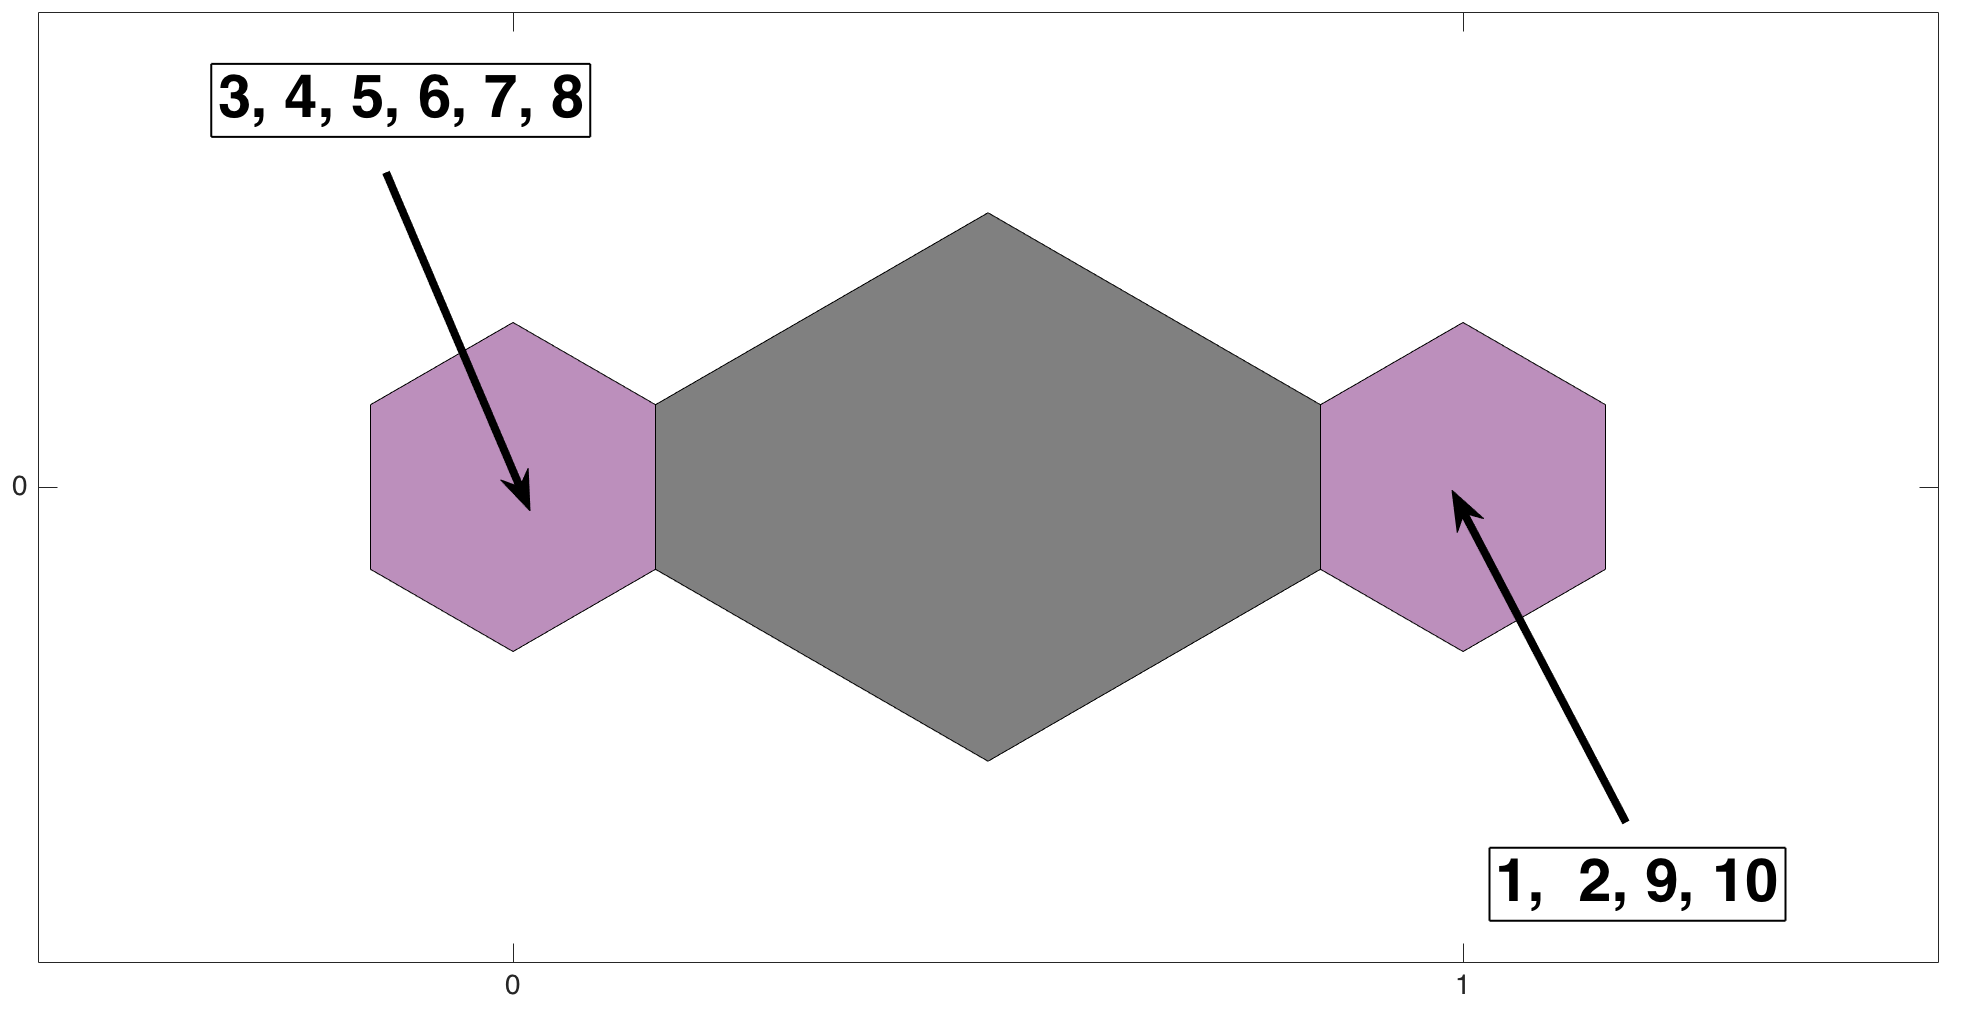
\includegraphics[width=0.5\textwidth]{../images0.01/M31/1D/combine_1D_1by2_all.png}
             }
            \hfill
            \subfloat[$1\times3$~network\label{fig: M31_net_1by3}]{
            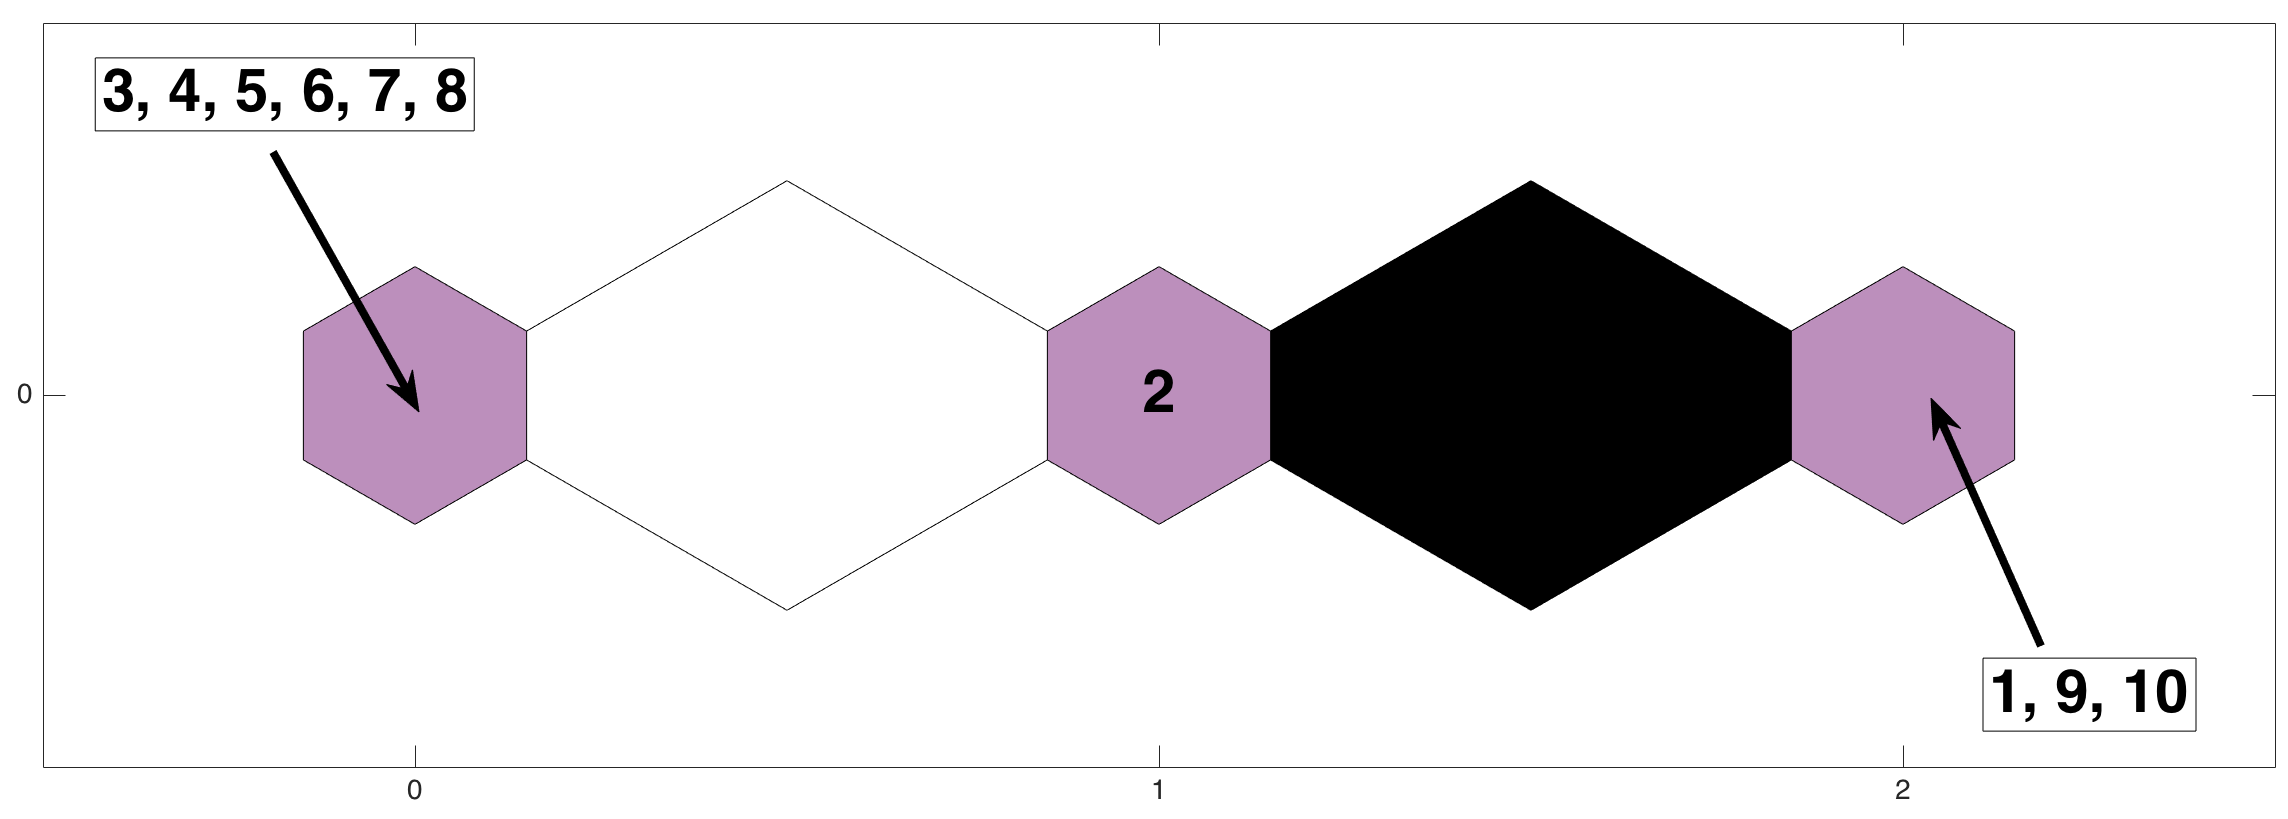
\includegraphics[width=0.5\textwidth]{../images0.01/M31/1D/combine_1D_1by3_all.png}
             }
             \hfill
            \subfloat[$1\times14$~network\label{fig: M31_net_1by14}]{
             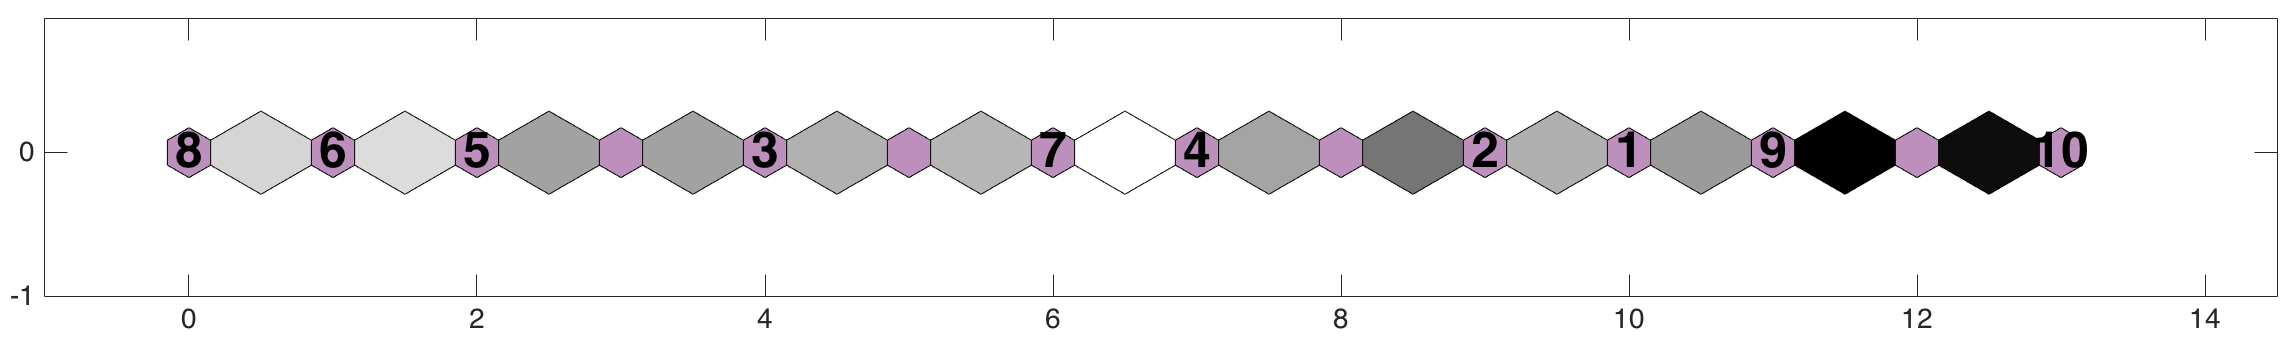
\includegraphics[width=0.5\textwidth]{../images0.01/M31/1D/combine_1D_1by14_all.png}
             }%%% What should I do with this one! It doesn't look good visually
            \caption{SOM of the M31 data from $1\times2$~, $1\times3$~and $1\times14$~grids. The axes show the position of the neurons. The purple Hexagonal shapes represent the neurons. The grey cycle colours show the differences between weight of each neuron with white is the minimum differences and black has the maximum one. The numbers in the plot show the regions that are located in each neuron.}
            \label{fig: M31_nets_1d}
        \end{figure}
        
        %%Network 1by14
        The network with 14 neurons, in Fig.~\ref{fig: M31_net_1by14}, is the first network which has no neurons with more than one region.
        Since at least 14 neurons are needed to separate all the 10 regions in M31, we can conclude that some of the regions have very small differences.
        In fig.~\ref{fig: regions in m31}, some the regions are grouped next to each other in the galaxy, which is the reason why some of the regions have vary similar input values.
        In Fig.~\ref{fig: M31_net_1by14}, the most right neuron is occupied by region 10.
        Two black colour between this region and the others indicates the high differences between this neuron and the other ones.
        The region 10 is located in the bulge of M31, and its separation from other regions, which are mostly located around of the inner or outer rings, is due to the fact that most of the input values for this region is much higher than the other regions.
        The region 8 occupies the most right neurons in this network, that suggests that this region has the most differences with the region 10.
        
        
    \subsection{Correlations}%%% I will find better title for this subsection
        %What is going on in this section
        Using SOMs, we can identify hidden subgroups in our samples. %%%% 
        Each of these subgroups were separated from each other, for a reason.
        This reason can vary from having higher values in some specific wavelengths, as discussed in Sec.~\ref{Sec: 1d_cluster}, to some unknown correlations between data, that cannot be seen in other groups or in a Galaxy's data as a whole.
        To investigate the later one, in Fig.~\ref{fig: cor_cluster1}, we plotted the Pearson correlation coefficients for the inputs from regions 3 to 8, which were clustered together in the $1\times2$ and $1\times3$ networks (see Figs.~\ref{fig: M31_net_1by2} and ~\ref{fig: M31_net_1by3}).
        
        \begin{figure}
        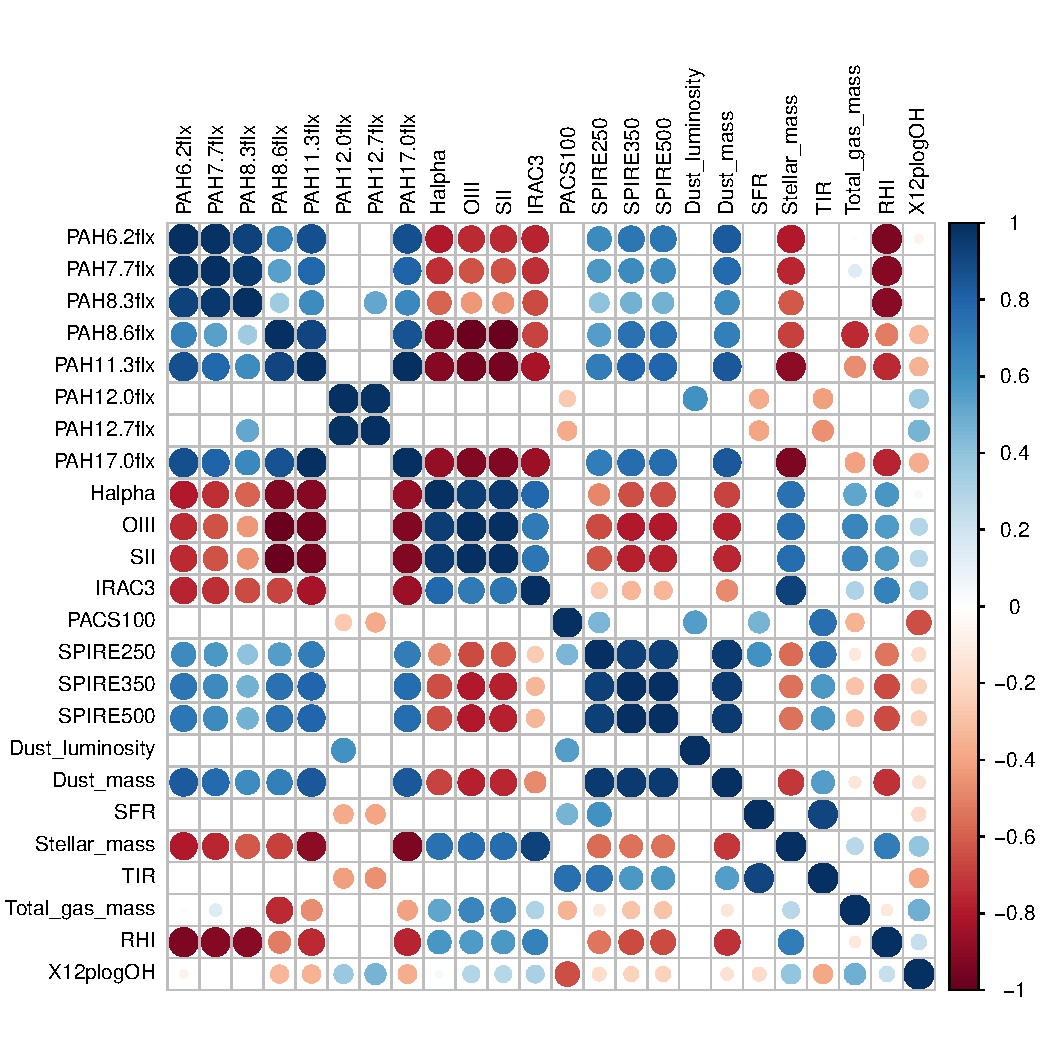
\includegraphics[width=0.5\textwidth]{../images0.01/cor_plots/M31_derived_3_to_8_core_plot_for_paper.pdf}%%% cut the white regions around the figure
        \caption{Same as Fig.~\ref{fig: cor_all}, but here we used data from regions grouped in the left side of the Figs.~\ref{fig: M31_net_1by2} and ~\ref{fig: M31_net_1by3}. }
          \label{fig: cor_cluster1}
        \end{figure}
        
        %%% what regions' version shows and how it compares with the other one:
        In Fig.~\ref{fig: cor_all}, are the PAHs fluxes correlates with each other. 
        Considering data from all M31 regions, There are very strong correlations between all the PAHs features and PACS~100~$\mu$m~, SPIRE 250 to 500~$\mu$m~emission, dust and TIR luminosities, SFR, and metallicity.
        However, in Fig.~\ref{fig: cor_cluster1},12.0 and 12.7~$\mu$m~ PAHs fluxes do not show any significant or strong correlation with PAH fluxes in other wavelengths or any other quantities.
        The only exceptions are the strong correlation between PAH flux at 12~$\mu$m and dust luminosity, and between 12 and 12.7~$\mu$m PAH fluxes.
        For the rest of the PAHs fluxes in Fig.~\ref{fig: cor_cluster1}, we cannot see any significant correlations with PACS~100~$\mu$m, dust and TIR luminosity, SFR, or metallicity.
        They also have weaker correlations with SPIRE emission than considering the case with all regions..
        However, further analysis showed that region 6 has higher amount of the SFR, and TIR luminosity, which causes the correlations between the PAHs, and SFR (or TIR luminosity) become insignificant. 
        By removing data for region 6, we can see high correlation between 6.2, 7.7, 8.3, 8.6, and 11.3~$\mu$m~PAHs features and SFR (and TIR luminosity).
        In Fig.~\ref{fig: cor_cluster1}, 6.2, 7.7, 8.3, 8.6, and 11.3~$\mu$m~PAHs features show strong anti correlations with RHI, stellar mass, \halpha, \sii, \oiii, and IRAC~5.6~$\mu$m~emission.
        
        %%% What the differences means?!
        
        
        %%% comparing with other works.
        
